\documentclass{article}

\usepackage{authblk}
\usepackage{url}
\usepackage[square,numbers]{natbib}
\usepackage{amssymb,amsmath}
\usepackage[margin=1in]{geometry}
\usepackage{graphicx}
\usepackage{setspace}
\doublespacing

%\SectionNumbersOn
%\AbstractOn

\title{Exact Learning}
%\author{Benedict W. J.~Irwin}

\date{\today}
\begin{document}
%\bibliographystyle{harvard}

\author[1]{Benedict W. J.~Irwin}
\affil[1]{Machine Intelligence Group, Microsoft Research, Cambridge}
\affil[]{\textit {beirwin@microsoft.com}}


\maketitle

\begin{abstract}
We present a working machine learning method that can reverse engineer a wide class of numerical functions and write out an exact mathematical expression.

This can be used for automated hypothesis generation, compiling tables of identities, assisting researchers as they work in an augmented fashion and ultimately one step closer to artificial intelligence working an reasoning with the space of analytic functions and performing exact, analytic mathematical tasks, attempting to understand complex data in high dimensions for example from particle physics/etc..

We give many examples.
We also attach a substantial theory document in the supplementary information.

Goal : 1D and 2D / 3D examples.... Can we just fit a Lauricella function or similar...


Goal : Sparse data distributions?
Goal : Fitting with barely any samples/moments.
Goal : Connection of MGF to PDF/coefficients
Goal : CDF etc.

Goal : Tons of working examples.
Goal : Cumulant GF connection.

\end{abstract}

%\tableofcontents

\section{Bigger Picture}
How do we find the mathematical rules behind our data? Many scientific fields have plots, curves and distributions that are not yet assigned an equation. We develop a framework to learn \underline{exact} mathematical solutions from numerical output. This could help researchers solve problems without having to solve equations.
In the long-term, developing such methods could lead to fundamental discoveries about our natural world. Can we learn complicated rules of physics and chemistry by spotting known functions in the data, and from this derive new theories?
We find an analogy between this method and the equations for neural networks that are already used today that gives a new perspective on the meaning of network parameters in existing models and could lead to advances in understandable AI. 





We present a collection of mathematical tools and emphasise a fundamental representation of analytic functions. Connecting these concepts leads to a framework for `exact learning', where an unknown numeric distribution could in principle be assigned an exact mathematical description. This is a new perspective on machine learning with potential applications in all domains of the mathematical sciences and the generalised representations presented here have not yet been widely considered in the context of machine learning and data analysis. The moments of a multivariate function or distribution are extracted using a Mellin transform and the generalised form of the coefficients is trained assuming a highly generalised Mellin-Barnes integral representation. The fit functions use many fewer parameters contemporary machine learning methods and any implementation that connects these concepts successfully will likely carry across to non-exact problems and provide approximate solutions. We compare the equations for the exact learning method with those for a neural network which leads to a new perspective on understanding what a neural network may be learning and how to interpret the parameters of those networks.


\section{Introduction}
This document summarises around eight years of work and represents a large development on top of an earlier preprint which laid down the foundations and mathematical concepts for exact learning. As this work was never published, we have attached it as the supplementary information of this document. However, for brevity we will only focus on new developments in the main text that allowed the idea to actually work in practice. 







First we reintroduce the motivation and goals of exact learning:


We will consider how in a broad sense `machine-learning-like-techniques' (i.e. advanced function fitting), can help with these `exact learning' type problems. Specifically for this work, the problem description is: 
\begin{enumerate}
\item[A)] \textbf{`Given a high precision numeric output of an unknown multivariate function or distribution write the `human readable equation' for that function as output, where it is possible to do so."}
\end{enumerate}
The concession we are willing to take on this quite general goal is:
\begin{enumerate}
\item[B)] \textbf{`Given a high precision numeric output of an unknown multivariate distribution write the \emph{unique fingerprint} of the distribution.'}
\end{enumerate}

The key change in goal B) is the introduction of a `\emph{fingerprint}' of an arbitrary function as a well behaved and meaningful intermediate that can identify a distribution \footnote{We have focused on distributions for the time being for simplicity, but extensions to this method will cover functions which are not bound at infinity}. The word fingerprint is local to this text and should not be considered a general term. The goals A) and B) can be seen as reverse engineering processes for \emph{functions}. It might be helpful to first consider the analogy of reverse engineering for a simpler object such as a \emph{number}, something that is performed by tools such as Simon Plouffe's `inverse symbolic calculator' \cite{Plouffe1986} and other `inverse equation solvers' \cite{Munafo}. In these tools a user can enter a high precision number - e.g. 14.687633495788080676 - and the algorithm would return a plausible closed form solution - e.g. $\pi^2 + e\sqrt{\pi}$. Once the user has the solution, the hope is that a human expert could use that extra information to come up with further insights which would assist in the scientific understanding of both the solution and problem.\\ 

Figure \ref{fig:Outline} depicts an overview of the `exact learning' procedure for a \emph{function}. Throughout this work we cover the necessary tools to understand the steps in the blue boxes on the right-hand side of this figure. Goal A) corresponds to the bottom left box, and goal B) is the bottom right box. The numeric data are collected from a natural source such as a very high-quality experiment, but more likely a numerical solution to a computational problem, or equation, or simulation. The solution is numerically transformed to `fingerprint space' (blue) by using an integral transform. The regularity of the representation of many analytic functions in this space assists with the fitting of the `fingerprint' using machine learning techniques to an assumed, highly generalised form. To get back to the mathematical expression of the solved function an inverse transformation is taken from the  fingerprint space to the function space. For examples of problems that might be interesting to solve using this method, please refer to the supplementary information. \\

\begin{figure}[h]
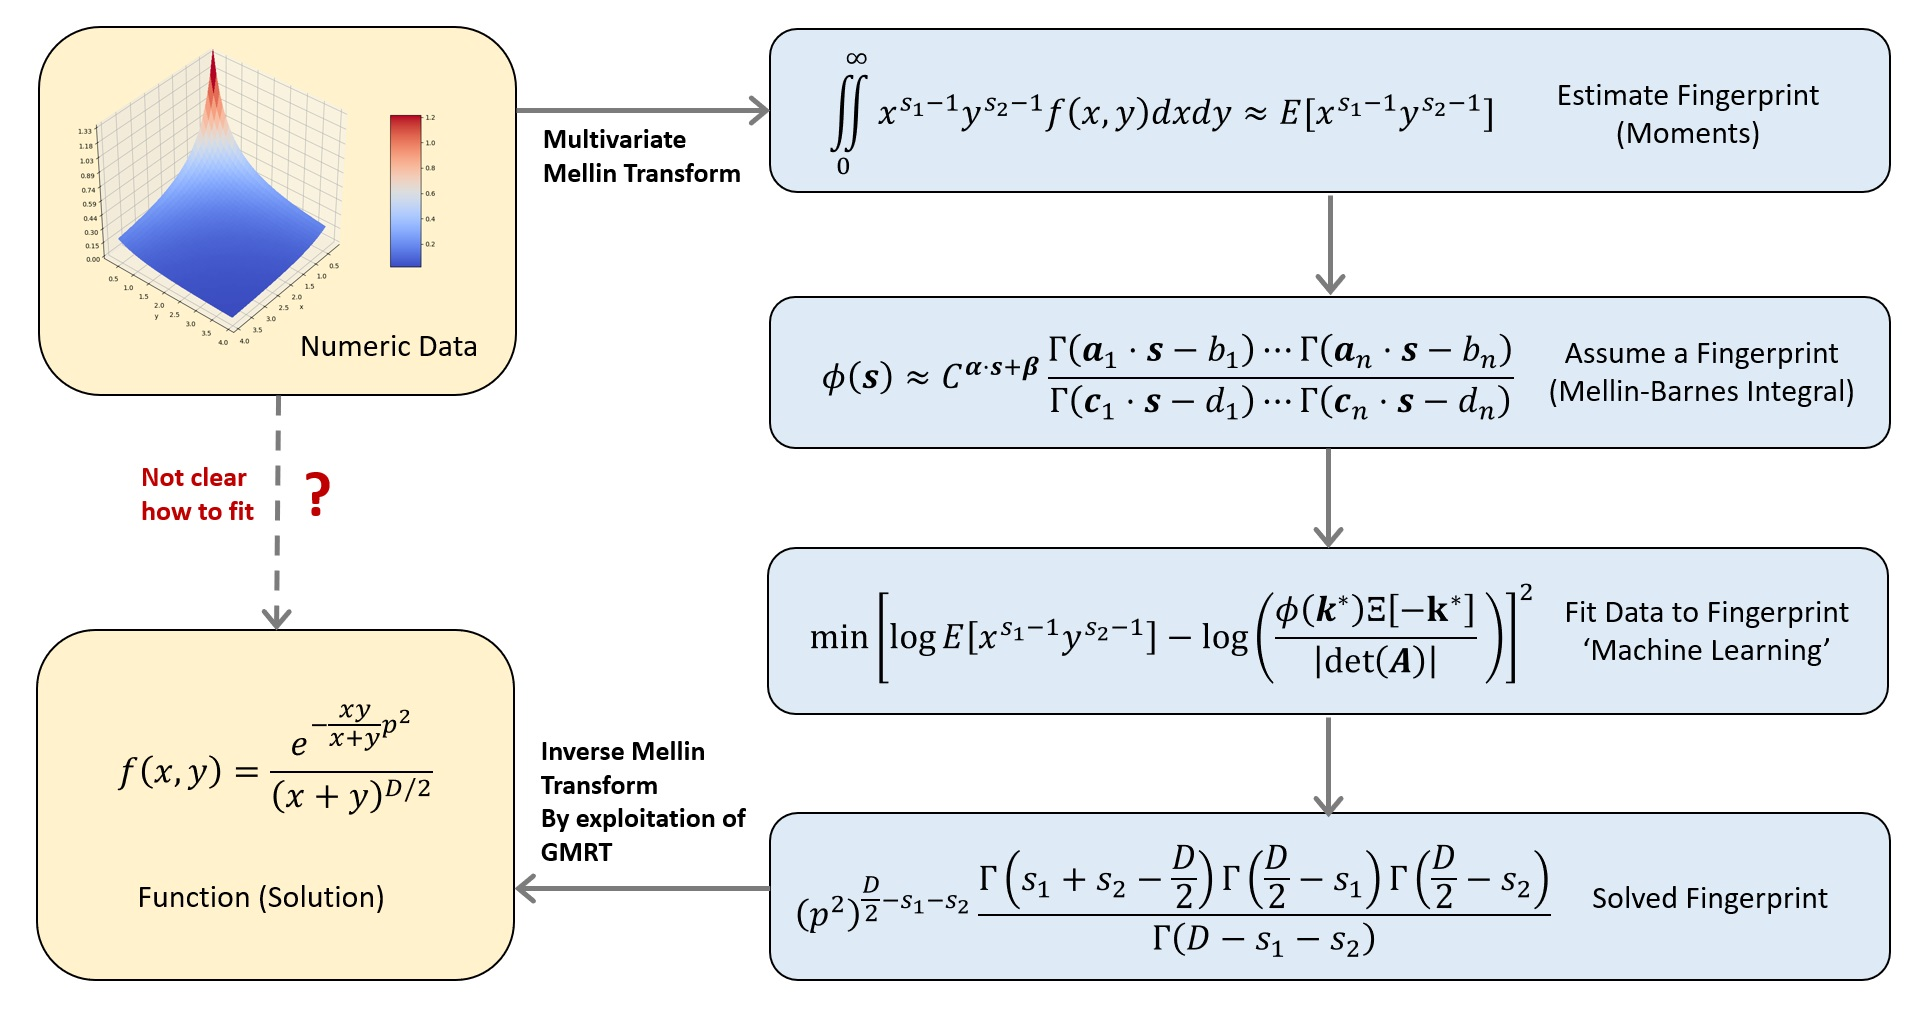
\includegraphics[scale = 0.323]{Figure1.jpg}
\caption{An example of the exact learning process, in this case with an example of the kernel of the massless Feynman bubble calculation given by Gonzalez et al. \cite{Gonzalez2015}. (Top left), A high precision numerical function is found as the solution to a problem that likely has an analytic solution, but the closed form is hard to derive mathematically. A numeric Mellin transform is made from the `function domain' (yellow) into the `fingerprint domain' (blue) for a number of chosen exponent vectors $\mathbf{s}=(s_1,\cdots,s_2)$. A highly generalised closed form for the fingerprint is chosen and then machine learning (function fitting) is used to track down the parameters of the function fingerprint ($\mathbf{a,b,c,d}$). With further analysis and interpretation of the solved parameters the fingerprint could be used to derive the closed form for the function that generated the original numeric data using the generalised Ramanujan master theorem (GMRT).}
\label{fig:Outline}
\end{figure}

\section{Theoretical Justification}
Unique moments : Discussion of three kind of moment problem $[0,\infty)$, $(-\infty,\infty)$ and $[a,b]$ with $[0,1]$ as a special case. Reference higher dimensional moment problem example. Try to link existence of CF via MGF via Mellin transform definition. Answer, if the moments converge, then the Mellin transform would converge, then the thing would exist, so they are unique... up to strip of holonomy?

Connection between coefficients, PDF, series coefficients MGF, CF, Mellin transform, cumulant GF.

Log-convex for many functions.

Solutions of differential equations. holonomic functions, annihilation operator, Mellin transform. etc.

\section{Multidimensional Examples}
Consider
$$
\mathcal{M}_D\left[\prod_{k=1}^n f_k \left(\alpha_k \prod_{l=1}^n x_l^{a_{kl}}\right) \right]=\frac{\prod_{k=1}^n \alpha_k^{-(A^\top)_k^{-1} \mathbf{s}}}{|\det(A)|} \prod_{k=1}^n g_k((A^\top)_k^{-1} \mathbf{s})
$$

Example
$$
f(x_1,x_2) = e^{-x_1+x_2}e^{-x_1 - x_2^2}
$$

\section{Sampling Strategy}
Some fingerprints are an analytic continuation from the convergent region of the sampling, i.e. sometimes moments don't exist. The theoretical expression and the sampled value may diverge beyond a certain boundary, and can be numerically slow to coniverge (for limited sample sizes) near the boundary. This effect makes certain values of $s$ inaccurate. However, it is easy to predict the values that are wrong... 

In the sample we have $x_min$ and $x_max$, thesmal


\section{Using Gradients}
We can sample the Mellin transform of the distribution as $\mathcal{M}[f(x)] = \phi(s) = E[x^{s-1}]$ however, using the property of the Mellin transform that gives the $k^{th}$ derivative of $\phi(s)$ as $\mathcal{M}[\log ^k (x) f(x)] = \phi^{(k)}(s) = E[\log^k(x)x^{s-1}]$. It turns out that a useful quantity to sample/fit to is the logarithmic derivative of the fingerprint in the series 
$$
\frac{d^0}{ds^0} \log \phi(s), \frac{d^1}{ds^1} \log \phi(s), \frac{d^2}{ds^2} \log \phi(s),\frac{d^3}{ds^3} \log \phi(s),, \cdots
$$
which are equal to 
$$
\log \phi(s), \frac{\phi'(s)}{\phi(s)}, \frac{...}{...}, \frac{...}{...}
$$
which can for the Mellin-Barnes class of functions be evaluated in terms of loggamma, digamma, trigamma, tetragamma functions etc.


Define $t_k = \phi^{(k)}(s)/\phi(s)$

$$
 \left\{\log (\phi (s)),\frac{\phi '(s)}{\phi (s)},\frac{\phi ''(s)}{\phi (s)}-\frac{\phi '(s)^2}{\phi (s)^2},\frac{\phi ^{(3)}(s)}{\phi (s)}+\frac{2 \phi '(s)^3}{\phi (s)^3}-\frac{3 \phi
    '(s) \phi ''(s)}{\phi (s)^2},\frac{\phi ^{(4)}(s)}{\phi (s)}-\frac{3 \phi ''(s)^2}{\phi (s)^2}-\frac{6 \phi '(s)^4}{\phi (s)^4}-\frac{4 \phi ^{(3)}(s) \phi '(s)}{\phi (s)^2}+\frac{12 \phi '(s)^2 \phi
    ''(s)}{\phi (s)^3}\right\}
$$
$$
\log (\phi (s)),t_1,t_2-t_1^2,t_3+2t_1^3-3 t_1 t_2,t_4-3t_2^2-6t_1^4-4t_3 t_1+12t_1^2 t_2
$$




\section{Sampling Effectively}
Real and imaginary deviance from distributions. Identifying the region of convergence via bounds of $x_min$ and $x_max$. [TO DO, linear interpolation of CDF and root finder for sample generation of optimal $s$ vector.]





\section{How Exact Learning Works}
The fingerprint fitting procedure has some subtle aspects which should be understood before jumping to conclusions.


Coefficients inside the gamma functions are usually integers or rationals.
Gamma functions are log-convex for positive real part.

For distributions with infinite number of moments (light tails), we expect positive arguments to gamma functions. For heavy tailed distributions there are some aspects to consider [TO DO].


\subsection{Using Knowledge}
I.e. bound distribution etc.



\section{The Exact Learning Python Package}
The exact learning method revolves around having a sensible list of fingerprint signatures, which are then queried as a potential match to some numerical data. Because the signatures are analytically quite specific, only a few moments are needed to verify a distribution. This results in a loss function being minimized, and if the final loss drops suddenly to an all time low (usually of order $10^{-5}$), the algorithm will attempt to analytically resolve the match. 

The package has been configured to assemble a fast numerical function suitable for BFGS on demand given an input fingerprint guess.

\subsection{Using the Package}
There are two main steps to using the package.

Step 1:	Generating the data/distribution, selecting (complex) sampling points for moments, calculating $E[x^{s-1}], E[\log(x) x^{s-1}], E[\log^2(x) x^{s-1}]$. These are saved to files.

One could imagine essentially inputting code to generate the distribution, and working from that point onwards. For some problems, rather than direct sampling, the solution of a differential equation, or integration problem is input.


Step 2: Exact learning,
\begin{verbatim}
from ObjectOriented import *
EE = ExactEstimator("Disk_Line_Picking", folder = "Disk_Line_Picking")
fps = [gen_fpdict(['c','c^s','linear-gamma','linear-gamma','neg-linear-gamma','neg-linear-gamma'])]
for k in fps:
  print("Setting Fingerprint: ",k)
  EE.set_fingerprint(k)
  n_bfgs = 10
  for i in range(n_bfgs):
    EE.BFGS(order = 1)
    print("{}%".format(100*(i+1)/n_bfgs),flush=True)

print("Completed!")
EE.speculate(k = 4)
EE.cascade_search()
\end{verbatim}



\section{List of Examples}
To show the algorithm works for a wide variety of statistical distributions we cover many basic cases
\subsection{Basic Cases 1D}

\subsubsection{Exponential}
We generate a high quality distribution
\begin{verbatim}
x = np.random.exponential(size=100000)
\end{verbatim}

\subsubsection{Linear Ramp}

\subsubsection{$\chi^2$ Distribution}

\subsubsection{Beta Distribution}
\begin{verbatim}
360*x**2*(-x**3/6 + x**2/2 - x/2 + 1/6)*Heaviside(1 - x)
\end{verbatim}

\begin{tabular}{|c|c|c|}
\hline
Function Name & Result & Correct? \\
\hline
Expontial D. & $\exp(-x)$ & yes \\
Beta D. & & yes \\
Linear Ramp & & yes \\
\end{tabular}



\subsection{Advanced 1D Cases}

\subsubsection{Disk Line Picking}

\subsubsection{Square Line Picking}

\subsection{2D Examples}
Consider the two dimensional density
$$
f(x) = e^{-a x_1/x_2}e^{-b x_1 x_2^2}
$$
$$
 \frac{1}{3} a^{-\text{s1}} \Gamma \left(\frac{2 \text{s1}}{3}-\frac{\text{s2}}{3}\right) \Gamma \left(\frac{\text{s1}+\text{s2}}{3}\right) \left(\frac{b}{a}\right)^{\frac{1}{3}
    (-\text{s1}-\text{s2})}
$$


\subsection{3D Examples}


\section{Sparse Distributions}

\section{Solving Problems}

\subsection{Schr\"odinger Equation}

\subsubsection{Harmonic Oscillator}
$V(x) = \alpha x^2$
Multiple energy levels to consider...

\subsection{Anharmonic Oscilator}
Consider $V(x) = \alpha x^2 + \beta x^4 + \gamma x^6$.


\section{Future Developments}
Increased focus on bounded intervals.
Considerations for mixtures of distributions (i.e. a sum of holonomic functions is also holnomic), looking for separability in the operator.
Increased detection of higher functions, i.e. Heun functions.
Increased support for higher dimensional data.


\bibliography{bibliography}{}
\bibliographystyle{unsrt}


\end{document}